\newpage
\section{SYSTEM DESIGN}
\addcontentsline{toc}{section}{\numberline{} SYSTEM DESIGN}
\subsection{Data Flow Diagram}
\subsubsection{Level Zero}
\begin{figure}[h]
        \centering
        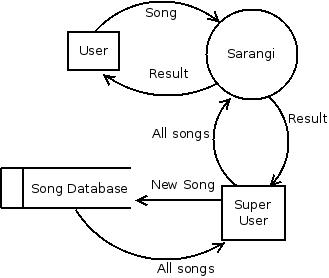
\includegraphics[width=75mm]{resources/contextlevel(0)}
        \caption{Context Level Zero}
        \label{fig:contextlevel}
\end{figure}
\subsubsection{Level One}
\begin{figure}[h]
        \centering
        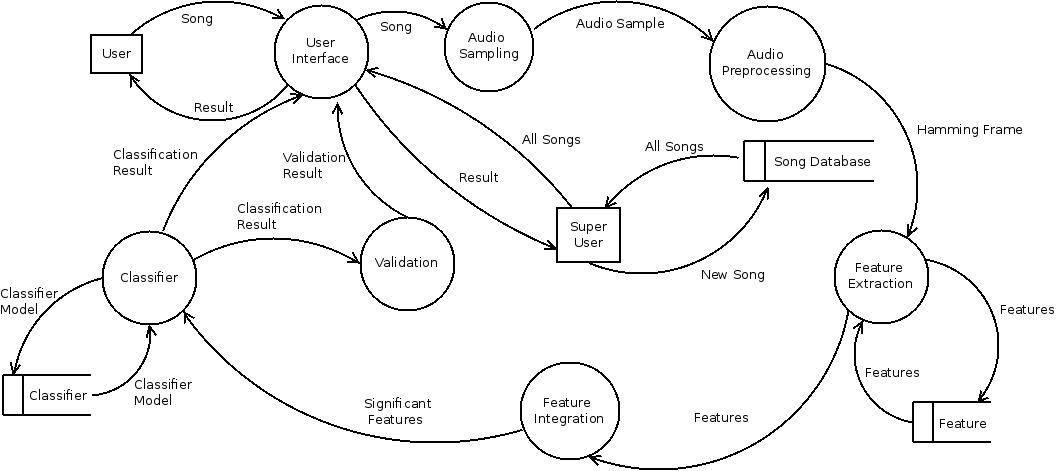
\includegraphics[width=173mm]{resources/level1b}
        \caption{Level One}
        \label{fig:level1b}
\end{figure}
\newpage
\subsubsection{Level Two}
\vspace{20mm}
\begin{figure}[h]
        \centering
        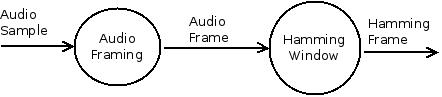
\includegraphics[width=150mm]{resources/preprocessing}
        \caption{Pre-processing}
        \label{fig:pre-processing}
\end{figure}
\vspace{20mm}
\begin{figure}[h]
        \centering
        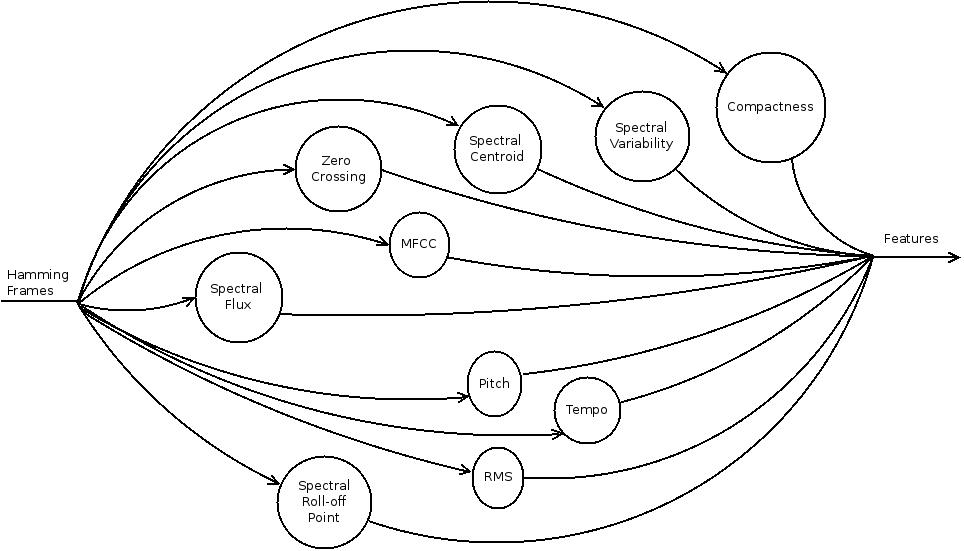
\includegraphics[width=150mm]{resources/feature}
        \caption{Feature}
        \label{fig:feature}
\end{figure}
\begin{figure}[h]
        \centering
        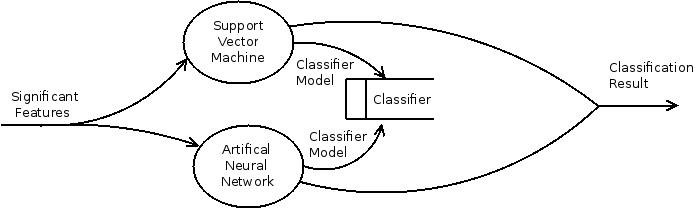
\includegraphics[width=150mm]{resources/classifier}
        \caption{Classifier}
        \label{fig:classifier}
\end{figure}
\begin{figure}[h]
        \centering
        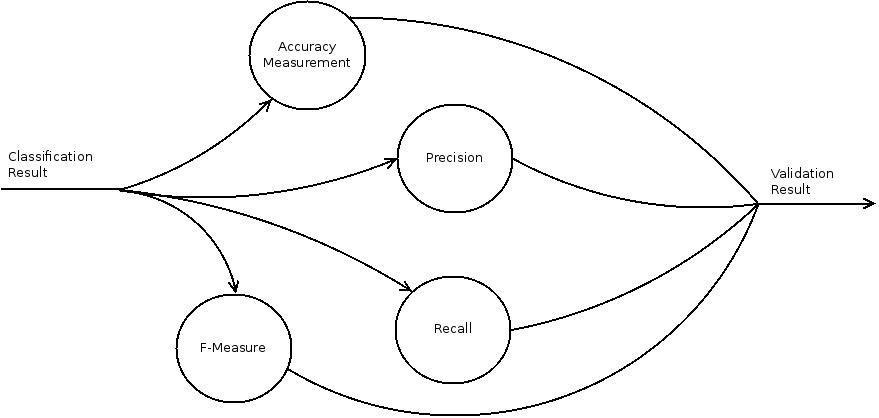
\includegraphics[width=150mm]{resources/validation}
        \caption{Validation}
        \label{fig:validation}
\end{figure}


